%!TEX root = ../projecto.tex
\section{Related Work} % (fold)
\label{sec:related_work}

This section provides insight of work done in multiple research areas that are related to the project. In subsection \ref{sub:self_organizing_maps} will be described multiple work done using Self-organizing maps. Subsection \ref{sub:topic_detection_on_twitter} is dedicated to work done on topic detection on the social network Twitter \citep{Twitter}

\subsection{Self-organizing Maps} % (fold)
\label{sub:self_organizing_maps}
Self-organizing maps are used in a wide are of applications, from authentications systems \cite{Dozono2012}, network intrusion detection \cite{intrusion_som} and speech recognition and analysis \cite{phonetic_typewiter}.

\subsubsection{Detecting Hidden Patterns on Twitter Usage} % (fold)
\label{ssub:detecting_hidden_patterns_on_twitter_usage}

\citep{Cheong2010} analyzed hidden patterns created buy the natural usage of twitter by its users. In its study they started by collecting data from the twitter API different kinds of topics like "2009 Iran Election" and "iPhone 3.0 OS launch". They made multi level signal extraction not only from information directly present on the tweet, but also by cross referencing with other social website and with the twitter user profile information. The signals retrieved from the social network can be seen in table \ref{tab:twitter_signals}.

\begin{table}[H]
  \caption{Twitter Signals}
  \label{tab:twitter_signals}
  \begin{center}
    \begin{tabular}{|l|l|l|}
    \hline

    \hline
    \textbf{Twitt Corpus} & \textbf{Twitter Profile} & \textbf{External Sources} \\
    \hline
       Tweet Size & Gender & Other Social Network Accounts\\
    \hline
       Replies & Number of customizations & Type of website\\
    \hline
       Re-tweets & Friends to followers ratio & \\
    \hline
       hashtags & frequency of posts & \\
    \hline
      \specialcell{Presence of URIs and \\ Type of linked content}
        & Account Age
        & \\
    \hline
       Type of Device & Country & \\
    \hline
       Tweet Location &  & \\
    \hline
    \end{tabular}
  \end{center}
\end{table}

By applying clustering algorithm of SOM, they could find 4 demographical clusters during the Iran 2009 Election. The first cluster was characterized by young web-based Iranians, with twitter accounts not older than 3 months with a high frequency of replies. The second cluster was mainly compound of web users from Iran accounts older that 3 months. The third cluster had Iranian users with mobile clients with large texts clearly trying to raise awareness. The fourth and final cluster represented the users around the world trying to raise awareness about the issue by sharing tweets with URIs.
Looking at their analysis about the topic "2009 Iranian Election" it is clear to see that it was possible to describe the type of users represented in the social network and the way they interact with it.

On the iPhone 3.0 OS launch it was possible to find three main clusters. The first cluster was characterized by male users, accounts older than 90 days, coming from countries where the iPhone is marketed, with high adoption of social media clearly representing the target market of the iPhone or its customers. The second cluster had new accounts with higher rate of followers to followees, high frequency of posts per day, presence of URI linking to technology blogs or websites, no country or gender specified meaning that this cluster was clearly composed by news aggregators and technological news websites. Inside the second cluster there was a subcluster of Japanese users which represents the high rate of iPhone adoption in Japan. Finally the third cluster was clearly spammer accounts that where eventually deleted after a couple of months, characterized by popular social connections, posting more than 50 tweets a day with external URIs and the accounts where not older than a day or so.

In conclusion it was possible to detect Twitter usage patterns and specifically detect spammers before they where banned from the social network. 
% subsubsection detecting_hidden_patterns_on_twitter_usage (end)

\subsubsection{Types of SOMs} % (fold)
\label{ssub:types_of_soms}

Depending on the kind of data that scientist are trying to analyze and visualize, different approaches can be made the SOM algorithm in order to better adapt to the data at hand.

Weight adaptation SOMs are simple Self-organizing maps in which the wheights of the vector space model are not even. For example \citet{Bacao2005}  proposed the adaptation of the algorithm in order to better represent geographical data where more weight is given to the coordinates of the data.

First introduced by \citet{multi_layer_semantics}, the Hierarchical SOMs are often used when it is possible to decompose on big problem into smaller problems. One or more SOMs are located at each layer usually operating in on different variables. The hierarchical SOM allows the creation of thematic classifications at lower layers which are then composed into a single one \citet{Bacao2005} which leads to a more specific kind of classification in the lower layers. 
Based on the survey made by their work \citet{Henriques2012} suggests that there are four main types of hierarchical SOMs, Thematic Agglomerative, Agglomerative HSOM based on clusters, static devised HSOM and dynamic devised HSOM.
Multi layered SOMs where used by \citet{Rauber2000} on automatically detect and organize topics in order to organize bookshelves. They used the vector space model to define all books and started initially with only four cluster, that where consequently sub-divided and categorized which in the end created a hierarchical tree of topics.
Multi layered SOMs have been used in a wide variety of applications, such as speech recognition \citet{multi_layer_semantics} and learning to control a robot arm and wrist \citet{Sayers1991}.


The Geo-SOM \citet{Bacao2005} applies the first law of geography “Everything is related to everything else, but near things are more related than distant things." to the SOM algorithm, where the winning neuron is chosen by in a radius k defined by the geo-coordinates of the data. In this way the Geo-som forces units that are close in the input space to be close in the output space. The representation of the Geo-som can be seen in figure \ref{fig:geo_som}.



\begin{figure}[tb]
  \begin{center}
    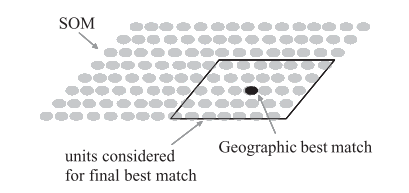
\includegraphics[]{images/6_geo-som.png}
  \end{center}
  \caption{Geo-SOM structure, from \citet{Bacao2005}}
  \label{fig:geo_som}
\end{figure}


Self organizing maps have their own limitations mainly drawing from the fact that it has a fixed number of neurons. \citet{Qiang2010} cites in his survey about the state of self organizing maps, that newer algorithms namely Growing cell Structures \cite{Fritzke1995} and Growing Neural Gas \cite{Fritzke1994} don't have this drawback.
% subsubsection types_of_soms (end)

% subsection self_organizing_maps (end)


\subsection{Topic Detection on Twitter} % (fold)
\label{sub:topic_detection_on_twitter}
% subsection topic_detection_on_twitter (end)
% section related_work (end)


\begin{itemize}
  \item What did we know about the problem before I did this study? 
  \item What did we do different from previous works? 
  \item Discuss the relevant primary research literature 
  \item Works should be organized by their relevant characteristics 
  \item Comment on why it is relevant for your work 
  \item Comment on what your work does differently 
\end{itemize}